\documentclass[10pt,journal]{IEEEtran}
\usepackage{ctex}
\usepackage{amsmath}
\usepackage{comment}

\begin{document}
\title{通过端口间缓存和vc共享技术改进路由器性能}
%\onecolumn
%\author{\IEEEauthorblockN{Baoliang Li}}
\author{Baoliang~Li, %~\IEEEmembership{Student Member,~IEEE,}
        Zeljko Zilic, %~\IEEEmembership{Senior Member,~IEEE,}
        Wenhua~Dou, %~\IEEEmembership{Non-Member,~IEEE}% <-this % stops a space
\thanks{Baoliang~Li and Wenhua Dou are with the College of Computer Science, National University of Defense Technology, Changsha 410073, P.R. China}%
\thanks{Zeljko Zilic are with Department of Electrical \& Computer Engineering, McGill University, Montreal H3A-2A7, Quebec, Canada}%
\thanks{Manuscript received XX XX, 2014; revised XX XX, 2014.}}

\markboth{Journal of XXX,~Vol.~XX, No.~XX, XX~2014}%
{Li \MakeLowercase{\textit{et al.}}: 端口间缓存和vc共享技术研究}

\maketitle

\begin{abstract}
实际的traffic负载在片上网络中的分布通常是不均匀的而且是动态变化的,处于low traffic load的端口/区域只需要较少的虚通道和缓存空间,而处于high traffic load的端口则需要较多的缓存空间和虚通道才能减少流量控制阻塞和HoL。传统的虚通道虫孔交换的片上网络路由器每个端口的虚通道和缓存资源都是静态分配的,无法适应这种流量的动态变化和多样性。为了迎合这一需求,本文提出了一种端口间缓存和虚通道动态分配的片上网络体系结构。该结构的两个重要的properties是:(1)可以在运行时动态的分配缓存和虚通道资源来适应网络流量的变化,以此来提高性能和缓存利用率;达到以较少的硬件资源来实现较高的性能的目的;(2)我们提出了影子vc的概念和虚通道组织方式,并以此来降低虚通道分配器和交换机分配器的规模;实现减少路由器流水线的关键路径长度的目的。experimental results on a 45nm CMOS standard cell library show that our architecture improve the performance of router by xx\% under bitcom, bitrev, etc. traffic pattern. 

\end{abstract}
\begin{IEEEkeywords}
Networks-on-Chip (NoC), buffer sharing,VC sharing
\end{IEEEkeywords}

\section{Introduction}
随着芯片集成度的提高,单个芯片上所能使用的晶体管数量大幅提高,同时过去通过提高主频来单核性能的方法受到散热和功耗的影响已经无法奏效。通过片上集成大量的处理器核的方法来提高性能是处理器设计的唯一出路。在多核和众核处理器系统中,核之间的通信由互连网络来实现。对于大规模系统片上网络提供了一种可扩展高性能低成本的实现方式。

缓存容量和组织方式是片上网络设计的重要方面,因为它会直接影响到整个片上网络的性能、功耗和成本。较大的缓存容量可以在高负载情况下减少流量控制造成的性能开销,但是会占用更多的芯片面积和消耗更多的能量。传统的虚通道虫孔交换的片上网络路由器为每个端口分配相同数量的虚通道并为每个虚通道分配同样大小的缓存空间\cite{DaTo01}。这种静态分配的路由器结构虽然实现简单,但是其缓存资源在某些特定的流量模式下,由于以下两个原因而得不到有效的利用:(1)不同端口实际需要的缓存资源不同;(2)同一个端口内的不同虚通道实际需要的缓存资源也不同。再画2张图表示每个端口实际需要的缓存数量是随时间变化的,并试图说明存在的以下两人个问题:(1)3x3 mesh的例子说明端口之间的利用率不平衡;(2)同一个端口内VC之间的利用率不平衡。与此同时,片上网络所占用的芯片面积和功耗比例越来越大\cite{1650108}。而且片上网络60\%的片上网络功耗是由缓存消耗的\cite{ChPe03}。

为了实现以较低的硬件成本和功耗实现较高的性能,研究者们提出了一类动态缓存分配的片上网络方案,例如\cite{NPKV06}\cite{4555894}\cite{5770788}\cite{Neishaburi:2009:RAN:1531542.1531658}\cite{6310960}。在这类体系结构中,路由器的每个端口仍然有相同数量的虚通道,但是每个虚通道所使用的缓存空间则是动态分配的。以3x3的mesh网络为例,在热点流量情况下(中间节点为热点)来说,热点的N和S端口接受的流量是W和E的3倍。因而如果能让W和E端口使用更多的buffer,那么那么对于因减少流量控制造成的stall而引起的大的延迟是非常有好处的。为了防止某些病态流占用所有的空间,最理想的办法是令每个端口使用$B_p=B_{total}\times\frac{C_p}{\sum_{p=1}^NC_p}$的buffer.然后对于每个端口所能使用的$B_p$个slot进行动态的管理。此外,端口间的buffer共享还有利于改进公平性以及不同数据流的吞吐率。

然而,光有动态缓存管理和端口间缓存共享通常是无法最大化片上网络的性能的。画一个图说明光有缓存动态管理和端口间共享是不够的,似如2个端口的所有vc都向同一个输出端口转发报文。vc是维持报文内部切片以正确的顺序传输的有效手段。如果因为某些原因,已经分配了vc的报文因某些原因被阻塞而无法前进,那么此时即使没有分配到vc的报文在前方没有阻塞也不能朝前,因为他没有可以使用的vc。另外在这种情况下,下游的缓存也将被闲置。因虚通道分配失败而造成的性能开销要比缓存不足引起的流量控制阻塞造成的开销大很多,特别是当报文长度很长时,因为只有当该端口有一个被占用的vc被释放,才有可能结束阻塞过程。由于虚通道是复用物理通道提高吞吐率的,为了防止报文交叠,只有当某个报文的尾切片已经写入buffer以后才能被分配给新的报文使用。因此某个端口实际需要的虚通道的数量等于该端口所要容纳的不完全报文的数量。因此,片上网络中不同的端口所需要的虚通道数量是随机流量模式和时间动态变化的。画一张图表示每个端口需要的虚通道数量。做实验时假设虚通道数量任意多,然后测量每个端口在不同的流量模式下实际使用的vc数量。

因此,只有在vc数量够用的情况下,实现端口间和端口内的缓存动态管理才能够从根本上提高和改进buffer的利用率,以实现用最少的buffer来实现最高的性能。之前的方案中\cite{NPKV06}\cite{4555894}\cite{5770788}\cite{Neishaburi:2009:RAN:1531542.1531658}\cite{6310960},为了保证最差情况下的虚通道需求,通常为每个端口设置非常大多的虚通道数量。由于存在大量的虚通道,使得vc仲裁器和sw仲裁器的实现非常复杂,也进一步限制了片上网络所能达到的工作频率,因为这两人个阶段通常处于片上网络时钟的关键路径上。另外,由于虚通道的规模可以保证在最差情况下的性能,在实现运行过程中这两个仲裁器的端口的利用率是非常低的。画图说明。

因此,设计合理的方案来动态的分配和管理虚通道是对改进性能非常有帮助的。为此,我们在本文中提出一种新的片上网络体系结构,即通过端口间动态共享vc来降低每个端口的报文因vc分配失败造成的阻塞和停顿,进而降低平均端到端延迟提升吞吐率。我们的方案采用部分动态的VC共享方式,每个端口分配一定数量的容量较小的静态VC,端口之间共享一定数量的动态VC。我们方案对上述几个问题的解决方法:(1)当某个端口的流量较少时,静态分配的VC足够支持切片数据的无阻塞移动。而当某些端口的流量较多时,共享的buffer则可以用来缓存大量的切片。(2)由于静态分配的VC相当于是为每个端口预留的配额,因而可以有效的避免共享缓存被某个端口耗尽时对低速端口的影响。(3)为了减轻VCA段的压力,我们提出了影子vc的概念,使得可以用较小规模的仲裁器来实现对大量vc的仲裁,进而提高了vc和sw仲裁器的利用率和最高工作频率。(4)我们所有的新增的硬件都可以并行的独立的操作,因而不对路由器的关键路径产生不利的影响。另外,我们的方案基于传统的路由器结构进行修改得到,不需要像vichar一样对整个路由器结构进行重新设计和实现。inter-port buffer and vc sharing是我们论文的主题。本文的一个重要的目标是改进现在的NoC的buffer利用率,增强性能的同时避免不可接受的硬件开销以及影响关键路径。我们的设计的目的在于同时不引入较大的硬件开销。

本文余下章节的安排如下:第\ref{related}节介绍相关的研究现状,第\ref{implemented}节介绍我们提出的路由器体系结构,相关的实验结果在第\ref{experiments}节给出。最后,我们在第\ref{conc}节对本文进行总结。

\section{Related Work}\label{related}
有研究表明,input buffers account for a large fraction of the overall area and power budget of typical Network-on-Chip,而且存储一个报文消耗的能量要多于在链路上传输所消耗的能量\cite{1012681}。因此,减少缓存容量并提高缓存利用率是在保证性能的前提下降低片上网络功耗和实现开销的唯一办法。Proper buffer sizing and organization are essential to increase buffer utilization. 静态的缓存分配方法使得在不同的流量模式下,大量的存储资源得不到有效的利用。为了改进提高缓存利用率并提高性能,一些虚通道动态缓存分配的体系结构已经被提出。

Virtual Channel Regulator (ViChaR) was proposed in \cite{NPKV06}, which utilize a table based unified buffer structure to dynamically allocate the buffer resource for each virtual channel according to the traffic condition. TAMS的硕士论文中指出,ViChaR的方式提高了一个端口内部的buffer利用率,但是也提高了设计的复杂性和功耗。 A novel Dynamically Allocated Multiple Queue (DAMQ) was proposed for NoC systems \cite{liu2006shared}, which provides the same performance while keep the hardware cost very low. To eliminate the additional three-cycle delay of conventional DAMQ, a prefetch mechanism for DAMQ is proposed in \cite{6310960}. In \cite{4555894}, the authors proposed an linked list based buffer structure and a congestion avoidance scheme to improve the network performance and reduce the power and area cost of NoC. 前面提到的方法只解决了端口内的缓存区动态分配问题,  in \cite{Neishaburi:2009:RAN:1531542.1531658}\cite{5770788}, Inter-port buffer sharing was proposed to further improve the buffer utilization of entire router. 其中,MH提出的RAVC方法虽然支持动态VC容量以避免HoL,但是控制罗男过于复杂,硬件成本过高,需要大量的额外的存储器和寄存器文件来存储控制信息,而且RAVA的方法基于Vichar的方法,只能用于固定报文长度。 Accordingly, An similar inter-port buffer-stealing scheme for the normal router without VC was proposed in \cite{5722177}. To avoid addition control cost of fine-grained buffer sharing, a Partial Virtual Channel Sharing NoC (PVS-NoC) is proposed in \cite{5739053}. 该方法假设某些路由端口之前有一部分FIFO是可以被两个端口共享的;An Virtual Channel Renaming mechanism is proposed in \cite{6296442} for NoC to virtualize the physical VC and increase the robustness of NoC in case of failure.另外,为了避免一个病态的数据流占用较多的缓存空间而引起的性能下降,an adaptive backpressure机制在\cite{BeckerJMD12}中提出。对于端口间的动态缓存管理,还有一类粗粒度的共享方法,该类方法采用较多的分布式buffer来模拟输出缓存的交换结构\cite{Soteriou:2009:HDS:1591872.1591936},但是其设计目的是提出吞吐率,其缓存利用率和功耗效率很低。

另外,这类动态VC分配方案的本质是为每个端口分配大量的VC,并实现同一个端口内的不同VC的动态缓存分配(为了防止死锁,每个VC需要至少保留一个缓存空间,剩余的缓存空间则可以在不同的VC之间进行动态的分配。) 实际上,造成VC阻塞的原因是大量不完整的报文(即尾切片还没有到达)占据了所有的VC。存在大量不完成报文的原因主要是因为阻塞造成的同一个报文的不同的切片跨跃存在于几个路由器中。换句话说,这些路由器中都会有一条VC被该报文所占据而无法被其它报文所利用。由于不同端口的流量情况不同。但是,某个端口的不完全报文的最大数量等于于上一级的所有路由器中需要向该路由器注入流量的VC的总数。另外,在X-Y路由条件下,X方向更加容易拥塞,这种不均衡也导致之前的均匀分布vc的方案存在很大的问题。VC保证在同一个通道中的报文切片顺序不会交错。如果同时结合了动态缓存管理和虚通道管理,那么便可以使用有限的硬件资源同时降低流量控制阻塞,交换机分配阻塞和虚通道分配阻塞。这对于改进系统的性能是非常有益处的。本文中我们便实现了这样一种方式。 

\section{路由器体系结构}\label{implemented}
\subsection{Key architectural Conribution}
为了以较低的成本增强典型片上网络的性能,我们必须提高缓存的利用率,这就需要我们能够对路由器内部每个端口以及每个端口中每个虚通道的缓存都进行有效的动态管理和共享。除此之外,我们需要提供较多的虚通道数量这样才能保证尽可能减少因虚通道不足引起的阻塞。在全文的主题上,我们的目标是通过动态的共享虚通道和缓存来提高吞吐率降低平均端到端延迟,而之前的很多方案都是单纯的提如何提高缓存利用率并降低延迟。在具体的实现过程中,我们还要在实现的复杂度和资源的利用率之前进行折衷。

当需要进行VC间缓存共享时,通常的情况是这个端口已经很堵,因则借助端口内的缓存共享来改进性能的性能提升已经非常有限,而端口间缓存共享则没有这个问题。因为应用通常会呈现出流量在同一个路由器的不同端口间的不均衡分布情况,因而采用端口间共享对改进吞吐率有好处。

\subsection{提出的微体系结构}
为此,我们提出了该体系结构,如图所示。该体系结构包含以下几个重要的模块。1.流量控制模块:负责信约的生成、信约跟踪;2.共享buffer的监控模块,负责对共享缓存的虚通道的分配与释放,读写地址和控制信号的译码以及队列空满检测模块;3.拥塞的检测模块和共享buffer分配模块,负责对每个端口的拥塞状况进行动态的监控和对缓存的分配;4.虚通道和交换机的仲裁模块,负责在影子vc和实际vc之间的仲裁和分配。我们将在以下的小节中分别进行介绍。

我们的设计方案是在典型路由器结构的基础增加一些对共享缓存的控制和分配模块形成的。我们的方案为每个端口预留一定量的VC,然后剩余的VC被所有的端口共享。这样做的原因是为了为每个端口保证一定的吞吐率和带宽以避免当该端口出现猝发流量时没有可用VC的情况。预留不同数量的VC最终的性能是不同的,对于不同的流量模式可以进行多次实验找出最优的组合。这种部分虚通道共享方案对于热点流量效果会比较好,而热点流量又恰好对应于CMP系统中的MC或home节点。共享的buffer分成几个bank,用以支持动态的VC分配和端口间的缓存调整。这些共享的存储体每一个都独立的检测不同输入端口的流量状态(这些流量状态由若干个统计计数器来实现),并通过协商来确定每个存储体的分配方式以及分配的实际地址段。用若干个有限状态机来检测每个端口的拥塞情况并根据一定的策略动态的将空闲的bank分配给指定的比较忙碌的端口使用。在具体的实现过程中,我们可以动态的改进对指定Memory bank采用的控制策略,以适应不同流量模式的特点并提高其吞吐率。

为了支持这一改变,我们的方案中每个共享的bank输出5根线用于表示当前bank授权给评谁用。在路由器的每个输出端口上也有5根线用于表示这5个bank在该端口的可用性。信约控制模块也要进行相应的改变,每个端口增加N个信约计数器用于跟踪共享vc在当前端口的可用性。另外,还需要在每两个路由器之间增加两根信号线credit\_for\_shared用于表示当前反馈的信约是共享vc的还是私有vc的。为了标识每个输入的切片是否要注入实际vc还是影子vc,我们还需要增加1根输入信号线shared\_vc用于表明当前的vc id是针对私有vc的还是共享vc的。

总起来说,我们的方案与conventional router相比实现的性能提升源于以下四个方面:(1)实现了动态的vc分配,提高了缓存的利用率,可以利用较少的缓存资源实现同样的性能;(2)实现了vc分配器的共享,进而降低了va的复杂度和实现成本;(3)实现了端口间的vc共享,通过发现不同端口间对vc数量的不同需求和共享,我们的方案实现了端口间vc共享进而降低了因vc不足造成的阻塞;(4)我们的方案通过发现不同端口间对缓存容量的不同需要,动态的分配缓存资源到不同的端口,因而实现了资源的高效利用并以此来提高片上网络的性能。

\subsection{VC和SW仲裁器}
之前的方案仅实现了对缓存的动态分配和共享而没有实现vc的共享。然而我们发现因vc不足造成的阻塞要远远比缓存不足造成的后果要严重。考虑某种情况,当某条流在某个路由器中发生VC阻塞时,该条流会在路由器中积压大量的切片,而切片在缓存区中的积压会将该数据流转变成为恶意数据流。而且这种影响随着报文长度的增加而越发明显。造成这一现象的原因则是因为虚通道分配失败。

采用VC共享方案的本质原因是为了尽可以避免VC阻塞造成的性能下降。我们采用vc共享而不是像以前的方案一样为每个端口分配大量的虚通道的目的在于,受限于vc和sw分配器的实现复杂度,每个端口可用的vc数量是非常有限的。另外,受限于系统的设计成本,每个端口的缓存容量也是有限的。而系统所能达到的吞吐率与vc的数量以及缓存容量是正相关的,因此为了提高吞吐率需要较多的vc和缓存空间。但是不同端口的流量特点是不同的,在这种情况下,我们需要一种有效的机制来动态的共享vc和缓存并对其进行高效的分配和使用。

在我们提出的体系结构中,路由器的每个端口所能使用的缓存空间有两个部分,一部分是每个端口私有的缓存,这一部分缓存通过链表的方式动态的进行管理;另一部分为所有端口动态管理的缓存,这一部分缓存由有限状态机进行动态的管理和分配。为了避免写冲突,要求这些缓存空间被分成若干个小的存储体,这些存储体可以被并行的读写。共享的缓存区被分成5个或是5的整数倍数存储体,我们对vc的分配以存储体为粒度,当某个存储体被分配给相应的端口后,这个存储体上所有的vc也相应的分配给该端口。当属于某个端口的共享存储中所有的vc都空闲时该存储体便可以被重新分配。因此,每个端口所能使用的虚通道的数量是动态变化的。为了支持对最差情况下(即每个端口拥有最大数量的虚通道)的虚通道分配和交换机分配,一种可选的方法是为每个路由器配置一个较大的虚通道分配和一个较大的交换机分配器。但是,这样会使得整个系统变得非常复杂而且还会限制系统所能达到的时钟频率。

本文中,我们采用另一种新的方法。为此,我们提出了影子vc的概念。所谓影子vc是指那些属于共享缓存块的虚通道结构,为了限制虚通道和交换机分配器的规模,我们并不为这些影子vc预留专用的分配器端口,而是让这些虚通道复用私有vc的分配器端口。之所以称之为影子vc是因为我们的方案中影子vc与端口的私有vc共享同一个sw端口和va端口,这样即实现了对大规模vc的支持双降低了设计成本。而实际上这样的设计并没有降低系统的性能。因为被分配的VC在尾切片没有到达之前是不会grant任何请求的,分配器大部分时间都处于空闲状态,相应的端口可以被影子vc所使用。

与之前提出的动态vc分配的方案相比,我们的方案由于利用了分配器的复用技术,进而实现了利用较小的allocator来实现对大量vc的分配和使用,在很大程度上降低了allocator的实现成本并降低了关键路径长度,对于提高系统的主频非常有好处。这样一来,我们的VCA的实现电路得到了极大的简化,画一张图给出对应的电路设计方法。我们采用的影子VC技术也在一定程度上简化了VCA和SWA的实现。

关于VCA的实现,传统的方法在输入端采用V:1仲裁器,在输出端采用PV:1仲裁器;MH的方法输入端采用P个$V_{max}:1$ 仲裁器,输出端采用1个P:1仲裁器;而我们的方法,在输入端采用n个$V_i:1$仲裁器,其中($\sum_{i}^nV_i=V_{max}$),在输出端采用nP:1 仲裁器。采用几个小的仲裁器并行工作来代替一个较大的仲裁器的好处是降低硬件复杂度并易于提高主频。(考虑到同一个端口之间不需要进行匹配,能否利用n(P-1):1来代替)由于我们的方法在输入端有更多的请求胜出,因而更加有利于提高匹配的成功率。对于每个端口来说,每个时钟周期最多只有1个切片可以输出,因此只要分配一个输出vc即可以保证其吞吐率不受影响。由于我们的方法在VCA以及SWA上都有较高的匹配成功率,可以预见我们的路由器可以提供较高的吞吐率。每个下游节点的memory bank配置发生变化时都会通知VCA,VCA据此来屏蔽不能用的VC段。这样就不会存在冲突了。由于每个memory bank有独立的操控逻辑,因而我们支持的最大VC数可以比MH的方法要大。

同样的,我们的SWA也需要进行略微的修改。由于影子vc和私有vc共享同一个sw/va请求端口,因此我们需要在该端口上增加一个复选逻辑来选择一个请求输入到分配器中.修改后的sw仲裁器也是分为两人个附件,第一个阶段每个端口有1个5x/6:1的仲裁器用于从该端口中选择一个vc作为下一时钟的备选输出vc;另外,共享的5x/6个vc也有一个仲裁器,因此第一阶段我们有6个同样的仲裁器。第二阶段我们在每个输出端口放置1个6:1的仲裁器,用于从每一组仲裁结果中选择出一个vc进行切片传输可以看出,我们的sw分配器第二阶段采用5个相对较大的6:1仲裁器(原来的方案是5:1),但是在第一附件每个仲裁器的规模都比原来的方案要小(但是原来的方案需要5个我们的方案需要6个)。

在我们的方案中,为了简化VC分配逻辑,我们在Vc分配和sw分配时给影子vc赋预较高的优先级,以让其尽快排空队列,以缩短采用和整个vc的分配周期,尽可能快的适应当前网络的流量状况。

对于之前的共享VC方案,假设原来的动态VC方案中每个端口有x个VC,那么我们的方案每个端口设置5x/6个VC,另外还有5x/6个VC为各个端口间共享的。由于采用了影子vc和仲裁器端口复用,与之前的方案,对于同样的VC数量,每个VC仲裁器的复杂度则有所下降。由于我们实现了vc arbiter的复用,在我们的方案中,每个端口所能使用的vc数量在5x/6和10x/6之间,远远大于之前的设计方案,但是所用的vc分配器规模则远远小于之前的方案。我们的方案与vichar等方案的区别在于,尽管他们的vc也是动态分发的,但是没有实现端口间的共享。但是为了保证最差情况下的性能,每个端口都需要保存$V_{max}$个虚通道结构,vc,sw仲裁器也需要为$V_{max} \times V_{max}$规模以保证最差情况下的资源分配。而我们的方案只需要规模为$5/6V_{max}\times 5/6V_{max}$的分配器。

片上网络中的两个分配器实现很复杂,但是当报文很长时,空闲的时间会很多,因此通过对vc和sw分配器的复用可以获得极大的好处。定义一个指标来度量这一空闲度。$$\rho=\frac{\sum_{i=1}^N busycycles_i-\sum_{i=1}^Ninsufficientcycles}{N\times T_{totalcycles}}$$虽然我们的方法没有提高vc和sw分配器的匹配度(目前也有相关的研究),但是我们对每个分配器端口进行了复用,提高了其利用率,避免了闲置。达到了采用较少的vc和sw分配器实现了较大规模vc的分配目的。另外,由于每个端口可用的vc数量为$V_{min}$到$2V_{min}$之间,因而在一定程度上也缓解了因为vc分配失败所带来的开销。

\subsection{缓存分配模块的实现}
我们的共享虚通道技术为每个端口预留少量的VC以减少VC仲裁和分配的压力,为了保证最差情况下的延迟性能,我们需要一种技术来确定每个虚通道所需要的最少的buffer slot数量。这就是我们之前基于RTC的论文所要解决的问题,由于在动态VC共享方案中每个VC只需要保留1个buffer slot便可以保证无死锁。我们的方案采用RTC的方法来确定每个VC所需要分配的最少缓存区。对于热点流量来说,特别是热点处于mesh网络的四个角上或者四条边上的时候,热点路由器和一些其它的路由器总有某些端口的缓存是没有被利用的。不光这些缓存区是没有被利用的,就连这些端口所对应的VC也是无法被有效使用的。因此我们可以考虑共享一部分缓存区和VC,之前MH的方案中VC是每个端口所独有的,没有被共享;为了保证性能,需要为每个端口预留大量的VC才能保证性能。但是这无疑增加了硬件成本降低了资源利用率。共享缓存技术除了增加资源利用率以外,还增加了实现了动态VC分配中间出现的流量隔离技术。

集中的控制器根据每个端口的需要进行动态的分配,重新分配的前提是该共享存储体上的所有vc都空间(由于优先分配私有vc因此这种情况会经常出现)都已经被释放。每个集中的控制器提前若干周期预测每个端口的vc需求然后将vc回收的结果提前告知占用该vc的端口,在收到vc回收请求以后,该端口停止对相应共享vc的再分配,等该vc被排空后该端口向集中控制器告知该共享vc可以进行再分配。集中的控制器是一个有限状态机,该状态机负责对几个共享存储体的分配和调度,每个共享存储体有一个自己的状态机用于协调与各个端口的分配/回收请求。

采用一个有限状态机来控制对bank的分配,该状态机有3个状态。并设计一个公式来做为每个端口的请求度。对于5个bank和5个端口间的分配有25种方案,最优的方案由5个分配控制有限状态机来实现。

对共享缓存的分配算法如下:每个控制器中有5个计算器用于记录每个端口的相应vc段的分配情况,每个时钟如果该段vc均被分配且自增,当增加到最大值是暂停。当某个vc空闲时这一计算器清零然后重新计数。这个计算器将作为度量拥塞程度的指标。整个allocator是一个基于优先级的分配器,由于在水平方向容易发生拥塞「参考文献」,因此水平方向的两个端口优先级最高,只有当垂直方向更加拥塞时才将相应的共享存储块分配给垂直方向。我们的算法分为两个主要的步骤,第一步根据拥塞程度确定对应的memory bank应该是分配给水平方向还是垂直方向,第二步根据路由器所在的位置和每个方向的拥塞程度来确定分配给哪一个端口。整个分配器由一个有限状态机控制,共有3个状态,当两次分配的结果不同时中间需要有一个排空阶段,否则保持在分配阶段。对下一阶段的预测与这两个状态并行进行。

由于我们的共享存储模块是与路由器流水线并行工作的,不在关键路径上因此对系统的频率不会有影响。

\subsection{与其它几类方案的比较}
之后MH提出的端口间缓存共享的方案实际上实现了端口间的缓存共享,以减少因流量控制而造成的吞吐率下降和延迟增加。但是因为流量控制而造成的阻塞造成的影响相对虚通道不足造成的影响较小。我们提出的方案同时实现了端口间的缓存共享和虚通道共享,特别是端口间的虚通道共享对改进系统的吞吐率是非常有好处的,因为VC阻塞通常要较多的时钟周期。

另外,与之前MH提出的完全端口间缓存共享不同的是,我们的方案实现了部分端口间缓存共享。之前MH的方案还有下面的问题:由于每个端口的报文或者都存在一个memory bank里,或者与其它端口的报文存储在一起。这样的方法有以下问题:(1)去往不同端口的报文无法并行传输;我们的方案采用多个并行的存储体以减少这一影响。画图展示这一影响。实际上就是一种特殊的HoL。假设端口W到达的切片目的地为E和L,端口N和S都只产生目的端口为E的报文;在RR调度方式下,平均每3个周期服务1个W的E报文;而实际上,W端口中向L端口的切片在高度向E端口的切片时是无法前进的,由于读冲突的存在。

而我们的方案中每个端口所能使用的vc数量是动态变化的,假设虚通道的规模是NxN,那么我们的方案每个端口最多可以支持2N个虚通道。换句话说,对于同样的最大虚通道数量,我们的方案所用的分配器实际上只有以上两人个方案的一半。当然,这也不会影响性能,因为对于虚通道分配来说,由于每个时钟周期每个端口最多输出1个切片,因此只要能够保证每个时钟周期有一个输入虚通道被授权,就可以保证吞吐率。多余分配的虚通道在当前周期内是不会进行数据传输的。

我们的方法增加的硬件几乎都是简单的组合逻辑电路,因则硬件成本更低。由于我们采用可扩展的VC结构,因则降低了拥塞端口发生拥塞的可能,在一定程度上对避免HoL也有帮助。ViChaR和RAVC的方法都需要对整个路由器进行重新设计,因而成本高。而我们的新方法则主要是在原来的基础上增加了些硬件来提高buffer的利用率。

在硬件开始方面,对每个memory bank设置一1个存储控制模块这样使用的总的控制寄存器的数量要比为每个端口所有的存储体设置一个共用控制器要节省很多的硬件资源。因此,我们的方法从两方面节省了开销,一方面是几个小的控制器;另一方面是我们提出的混合式的存储管理方法的动态存储容量要比同等大小的完全动态的管理方式要小很多。因,最后可以画一张表并给出一张图列不这些比较的结果。

端口间的缓存共享可以提高buffer的利用率,使得采用较少的buffer实现较高的性能成为可能。虽然采用共享存储的方式增加了控制逻辑的复杂度,但是提高了性能和缓存利用率,以VichaR为例,实现同样的性能只需要传统路由器50\%的存储资源。但是,完全的端口间缓存共享(例如mh和mit女人)需要非常复杂的逻辑支持以及大量的硬件支持,而这些复杂的硬件又会进一步增加系统的功耗。mit的研究表明尽管共享提高了吞吐率但是功耗却大大增加这样也就在很大程度上降低了这类方案的可用性。我们的方案实际上是在不共享和完全共享之间的一个折衷,通过仅共享一部分缓存空间,我们使用对共享缓存的控制存储开销大大降低,列一个表给出我们的方案与mh方案需要的指针寄存器的数量。最终还可以列一个表给出我们的功耗与mit的方案比较的结果。而且之前的方案都是只共享了缓存而没有共享vc,当某个端口的vc全部被占用时我们的方案还可以借助其它端口的空闲vc。

MH的方案每个端口有一个较大的缓存器和一套控制逻辑,假设每个端口有B的缓存资源;那么free buffer tracker的开销为$B\times log_2 B$,header pointer 
的开销是$V_{max}\times log_2 B$,tail pointer的开销是$V_{max}\times log_2 B$,下一跳指针的开销$B\times log_2 B$;5个端口总的控制开销为$10\times(B+V_{max})\times log_2B$;
而在我们的方案中,由于总的缓存资源中有一部分会被独立分配给每个端口做为静态VC,而且剩下的动态缓存资源又被分为几个小的memory bank,每个memory bank需要的控制资源比较少,我们假设有一半的缓存分配给静态VC,那么我们的方法控制开销为$5\times(B+2V_{max})\times log_2(B/2)$;

另外,我们还可以与mh的方案进行比较,mh的方案为了实现buffer共享,每个端口的next buffer slot ,header ptr和tail ptr应该都是可以寻址到该路由器中任何一个buffer slot的。因此,这种共享方案的控制存储应该是非常耗资源的。对于缓存控制资源的比较:
我们的方案:
$5(2*5/6V_mlog5/6B+5/6Blog5/6B)+5/6BlogB/6+5/6BlogB/6$

敕的方法:
$5(2V_mlogB+BlogB)$

MH的方案1: 
$5(2V_mlog5B+Blog5B)$

MH的方案2:

\begin{figure}
  \centering
  % Requires \usepackage{graphicx}
  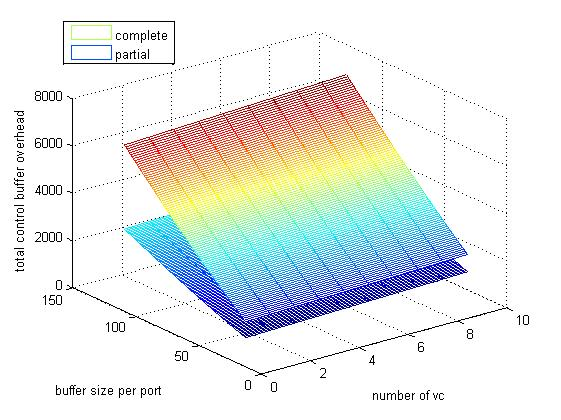
\includegraphics[scale=0.45]{figures/dynamic_vs_partial.jpg}\\
  \caption{完全动态与部分动态的比较}\label{comparions}
\end{figure}

通过这种方式,我们的方案所使用的控制存储资源要比mh小,同时我们的方案所用的控制存储资源实际上也比lai的方案要少。在做实验进行比较的过程中我们可以考虑两种情况:(1)同样的flit buffer大小的情况下比较性能; (2)同样的存储控制开销的情况下比较性能。(3)同样的性能情况下两人种方案需要的存储器和控制存储资源的多少。

\section{实验与评估}\label{experiemnts}
为了展示我们提出的体系结构的性能优势以及成本等特点,我们采用Verilog实现了一个时钟精确的noc路由器模型,该模型通过Synopsys工具进行综合,采用的工艺库是open-source process design kit FreePDK 45nm Standard Cell Library工艺[参考文献]。在做实验时可以考虑不同的报文长度以模拟cache一致性协议的需求,例如将报文长度取双峰分布,一个长度为1(对应读请求或者写响应消息)一个长度为16(对应cache行)。在具体的实现过程中,报文长度采用随机长度,每个缓存器的容量为x个切片,每个切片为64bit宽。每个端口共有10个私有vc,共享缓存共有10个影子vc。我们实现了基于虫孔交换的标准5段流水线的片上网络,采用基于信约的流量控制,路由算法采用维序路由,拓扑结构为Mesh结构。流量模型为均匀流量,bitrev, bit com, tornado以及热点流量等,热点流量恰是Cache一致性能及MC访问的重要应用场景。我们的方案在热点流量情况下可能很有用,效果会很明显。对于非均匀流量,特别是热点流量情况下,端口间的流量分布是严格不均匀的,因而我们的方案可能会得到更大的收益。

我们在做实验的时候还可以考虑这样一种情况:对于conventional router、damq路由器和我们提出的路由器结构而言,为了达到同样的性能,我们的方案在需要的缓存资源方面的节省情况。由于实现了端口间的VC共享,我们的方案还可以实现的另一个目标是减少每个VC仲裁器的开销。因为这个仲裁器通常处于路由器流水线中的关键路径上。为了采用较小的分配器来实现大量动态VC的分配,我们的方案要求每个输入端口要有一个VC分发逻辑。该逻辑还要实现VC的重定向以实现流量隔离,避免某个恶意数据流占据所有的缓存空间。缓存资源的使用比较:(1)列表比较资源;(2)实验比较性能,包括吞吐率和延迟;(3)综合结果比较面积和功耗。

实验结果如下:对于动态分配的片上网络路由器结构,对于同样的缓存容量,动态功耗为99.4796mW,芯片面积为827262.788363,而我们的方案功耗为101.8994mW,面积823642.608870.经过比较发现我们的方案功耗提高2\%,但是占用的芯片面积下降0.4\%.

在做实验的时候我们可以统计每个buffer的利用率。我们的方法对于均匀流量来说收益可能是负面的,原因解释与ICCAD'12上的论文相同。另外,counter\_width是一个额外的参数,考察其与系统性能的关系。

\section{conclusion and futher works}\label{conc}
我们提出的是一种运行的VC自适应技术,之前基于RTC的研究属于面向应用的buffer sizing方法,属于设计时的方法。在后继的研究中可以考虑在动态vc分配的基础上实现流量的隔离和服务质量保证。

\section*{Acknowledgement}
The authors thank the reviewers for their suggestions and comments, and all the experiments are carried out at the Integrated Microsystem Lab (IML) of McGill University. This research is supported by High Technology Research and Development Program of China (Grant No. 2012AA012201, 2012AA011902).

\bibliographystyle{unsrt}
\bibliography{Docear}
\end{document}
